\Chapter{Chapter 5}{Comparing one or two means}{Chapter 5: Comparing one or two means}

\fancyhead[R]{\fontsize{12}{14}\selectfont\textit{Chapter 5: Comparing one or two means}}

\chaptertitle{Chapter 5: Comparing one or two means}

\learningobjectives{
    \item Hypothesis testing by hand using the z- and t-score
    \item Generating and interpreting z-scores and t-scores
    \item Independent two-sample t-test by hand and in R
    \item Dependent two-sample t-test in R
}

% To add an assignment to the chapter, create a file in the folder "Assignments" and insert the link below

%%%%%%%%%%%%%%%%%%%%%%%%%%%%%%%%%%%%%%%%%%%%%%%%%%%%%%%%%%%%%%%%%%%%%%%%%%%
% Assignment 5.1: Hypothesis testing by hand using the z- and t-score
%%%%%%%%%%%%%%%%%%%%%%%%%%%%%%%%%%%%%%%%%%%%%%%%%%%%%%%%%%%%%%%%%%%%%%%%%%%

\handassignment{Assignment 5.1: Hypothesis testing by hand using the z- and t-score}

The maximum allowed amount of PFAS chemicals in soil is 0.9 microgram per kg of dry soil. In a regular soil check, researchers take 49 soil \concept{samples} in a town near a plastic factory and find a \concept{mean} PFAS level of 0.918 microgram/kg with a \concept{standard deviation} of 0.071. They want to show with 95\% confidence that the PFAS levels in the town are significantly above the norm. \\

\question{
    5.1 a
}{
    Write down the relevant information from this case.
}

\twolineanswerbox{5.1a}

\question{
    5.1 b
}{
    Write down the \concept{null hypothesis} $H_0$ and the \concept{alternative hypothesis} $H_1$ for the researchers’ test of the \concept{mean} PFAS level against the norm.
}

\hypothesesbox{5.1b}

The \concept{critical z-value} for a one-sided 95\% confidence interval is equal to 1.645 (see also Table 1 on page~\pageref{table1}) \\

\clearpage % Page break

\question{
    5.1 c
}{
    Calculate the \concept{lower bound} of the one-sided \concept{confidence interval} for the PFAS level \concept{population mean} with 95\% confidence.
}

\emptyanswerbox{
    5.1c
}{
    Lower bound: \shortanswerline
    \answerskip
    Calculation:
    \answerskip
    \rule{\textwidth}{0.4pt}
}

\question{
    5.1 d
}{
    Draw the conclusion for the researchers. Include the following four elements:
        \begin{itemize}
    \item[$\square$] Show how $\mu_0$ relates to the \concept{confidence interval.}
    \item[$\square$] Discuss whether $H_0$ is rejected or not.
    \item[$\square$] Describe what this tells us about $\mu$ and $\mu_0$.
    \item[$\square$] Describe what type of error is relevant \textit{(type-I or type-II)}.
\end{itemize}
}

\sixlineanswerbox{5.1d}

\question{
    5.1 e
}{
    Calculate the \concept{z-score} for this situation.
}

\hint{Hint 5.1: You can find the formula for the \concept{z-score} in the formula sheet. Use $\mu_0$ in this formula.}

\emptyanswerbox{
    5.1c
}{
    z-score: \shortanswerline
    \answerskip
    Calculation:
    \answerskip
    \rule{\textwidth}{0.4pt}
}

\clearpage % Page break

\question{
    5.1 f
}{
    Compare the calculated \concept{z-score} with the \concept{critical z-value}. What does this tell you about the \concept{p-value}?
}

\hint{Hint 5.2: Use the absolute value of the calculated \concept{z-score}.}

\twolineanswerbox{5.1f}

\question{
    5.1 g
}{
    Draw the conclusion again, but now using the \concept{z-score}, is it the same? Include the following elements:
    \begin{itemize}
    \item[$\square$] Show how the calculated \concept{z-score} relates to the \concept{critical z-score}.
    \item[$\square$] Discuss whether $H_0$ is rejected or not.
    \item[$\square$] Describe what this tells us about $\mu$ and $\mu_0$.
    \item[$\square$] Describe what type of error is relevant \textit{(type-I or type-II)}.
\end{itemize}
}

\sixlineanswerbox{5.1g}

The researchers want to quickly check another town near the plastic factory, but have less time available. They take 16 \concept{samples} in the second town and find a much higher \concept{mean} PFAS level of 0.930 microgram/kg with a comparable \concept{standard deviation} of 0.070. \\

\question{
    5.1 h
}{
    Calculate the \concept{t-score} for this situation.
}

\hint{Hint 5.3: You can find the formula for the \concept{t-score} in the formula sheet. Use $\mu_0$ in this formula.}

\clearpage % Page break

\emptyanswerbox{
    5.1h
}{
    t-score: \shortanswerline
    \answerskip
    Calculation:
    \answerskip
    \rule{\textwidth}{0.4pt}
}

The \concept{critical t-value} for a one-sided 95\% \concept{confidence interval} with 15 \concept{degrees of freedom} is equal to 1.753.

\question{
    5.1 i
}{
    Draw the conclusion for the researchers using the (absolute) t-score. Include the following elements:
    \begin{itemize}
        \item[$\square$] Show how the calculated \concept{t-score} relates to the \concept{critical t-score}.
    \item[$\square$] Discuss whether $H_0$ is rejected or not.
    \item[$\square$] Describe what this tells us about $\mu$ and $\mu_0$.
    \item[$\square$] Describe what type of error is relevant \textit{(type-I or type-II)}.
\end{itemize}
}

\sixlineanswerbox{5.1i}

\question{
    5.1 j
}{
    Also calculate the \concept{lower bound} of the one-sided \concept{confidence interval} for the PFAS level \concept{population mean} with 95\% confidence.
}

\emptyanswerbox{
    5.1j
}{
    Lower bound: \shortanswerline
    \answerskip
    Calculation:
    \answerskip
    \rule{\textwidth}{0.4pt}
}

\clearpage % Page break

\question{
    5.1 k
}{
    If you would draw the conclusion based on this \concept{lower bound} would you get the same result? Explain why.
}

\emptyanswerbox{
    3.4g
}{
    The conclusion \textbf{would} / \textbf{would not} be the same.
    \answerskip
    Explanation:
    \answerskip
    \rule{\textwidth}{0.4pt}
    \answerbreak
    \rule{\textwidth}{0.4pt}
}

\question{
    5.1 l
}{
    Why is it that even though the second town shows much higher PFAS level in the \concept{sample} (0.930 vs 0.918) $H_0$ cannot be rejected?
}

\twolineanswerbox{5.1l}

\clearpage % Page break
%%%%%%%%%%%%%%%%%%%%%%%%%%%%%%%%%%%%%%%%%%%%%%%%%%%%%%%%%%%%%%%%%%%%%%%%%%%
% Assignment 5.2: Generating and interpreting z-scores and t-scores
%%%%%%%%%%%%%%%%%%%%%%%%%%%%%%%%%%%%%%%%%%%%%%%%%%%%%%%%%%%%%%%%%%%%%%%%%%%

\rassignment{Assignment 5.2: Generating and interpreting z-scores and t-scores}

In assignment 5.1 you have seen that to calculate a 95\% one-sided \concept{confidence interval} for a \concept{sample} with $n \geq 30$ you need to use the correct \concept{z-value}. Now you are going to find out how to get that number from \texttt{R} using the \rcode{qnorm()} function. The \rcode{qnorm()} function returns the \rcode{x}-value for a certain probability for a specified \concept{normal distribution}, if you do not specify the \concept{mean} (\rcode{mean}) and \concept{standard deviation} (\rcode{sd}) arguments it returns the \concept{z-value} for the \concept{standard normal distribution}. \\

Run the following code in R: \\

\codeblock{qnorm(p = 0.95, mean = 0, sd = 1, lower.tail = TRUE)\\
{\color{dataset} \# Or because the standard normal distribution is the default simply use:}\\
qnorm(0.95)
}

\question{
    5.2 a
}{
    Round the number to 3 decimals. Do you recognise this \concept{z-value}?
}

\emptyanswerbox{
    5.2a
}{
    Result: \shortanswerline
    \answerskip
    \rule{\textwidth}{0.4pt}
}

In assignment 5.1 you have also seen that for the 95\% two-sided \concept{confidence interval} for a \concept{sample} with $n \geq 30$ you can use z = 1.960. Now you are going to learn to reproduce that number in \texttt{R}. \\

Run the following code in R: \\

\codeblock{qnorm(p = 0.975)}

\question{
    5.2 b
}{
    Why do you have to use the 97.5 percentile to get the z-value for the 95\% two-sided \concept{confidence interval}?
}

\twolineanswerbox{5.2b}

\clearpage % Page break

Run the following code in R: \\

\codeblock{pnorm(q = 1.645, mean = 0, sd = 1)\\
pnorm(1.960)
}

\question{
    5.2 c
}{
    Based on the results of this \texttt{R} code explain what the \rcode{pnorm()} function does.
}

\twolineanswerbox{5.2c}

In assignment 5.1 it was stated that the \concept{critical t-value} for a one-sided 95\% \concept{confidence interval} with 15 \concept{degrees of freedom} is equal to 1.753. \\

Run the following code in R: \\

\codeblock{qt(p = 0.95, df = 15)}

\question{
    5.2 d
}{
    Based on the results of this \texttt{R} code explain what the \rcode{qt()} function does.
}

\twolineanswerbox{5.2d}

Run the following code in R: \\

\codeblock{pt(q = 1.753, df = 15)}

\question{
    5.2 e
}{
    Based on the results of this \texttt{R} code explain what the \rcode{pt()} function does.
}

\twolineanswerbox{5.2e}

\clearpage % Page break

\begin{center}
    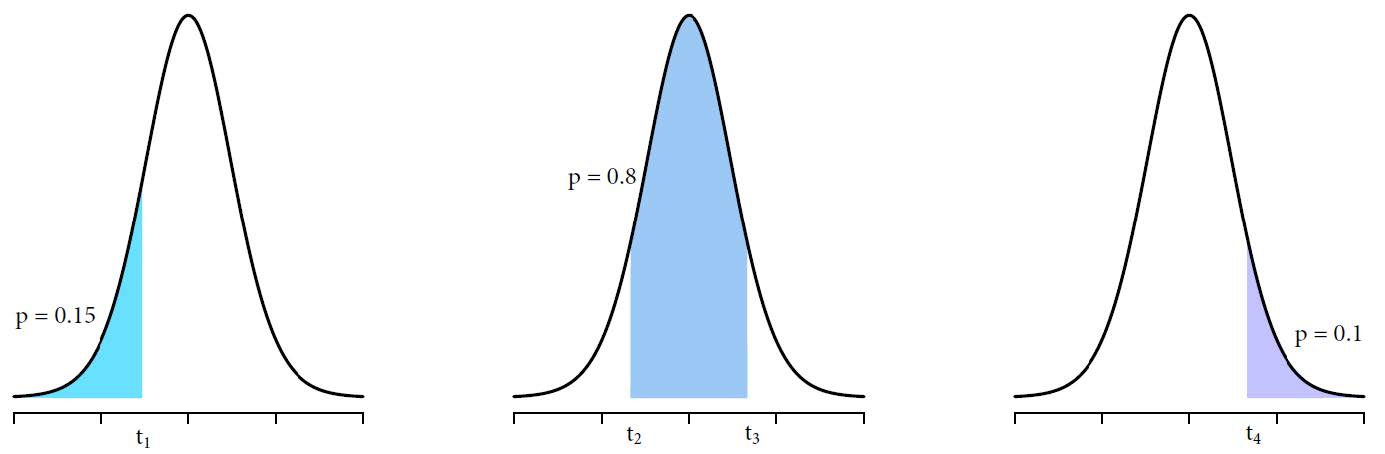
\includegraphics[width=\textwidth]{Files/Images/tdistributions2.jpg}
\end{center}

\question{
    5.2 f
}{
    For the situation where there are 19 \concepts{degrees of freedom}, use the \rcode{qt()} function to get the \concept{t-values} (t$_1$, t$_2$, t$_3$, t$_4$) for the three situations shown in the picture above.
}

\hint{Hint 5.4: For the picture on the right keep in mind that the \rcode{qt()} function by default returns the value for the left tail of the distribution.}

\rcodeanswermedium{5.2f}

\emptyanswerbox{
    5.2f
}{
    t$_1$: \shortanswerline \hspace*{3cm} t$_2$: \shortanswerline
    \answerskip
    t$_3$: \shortanswerline \hspace*{3cm} t$_4$: \shortanswerline
}

\begin{center}
    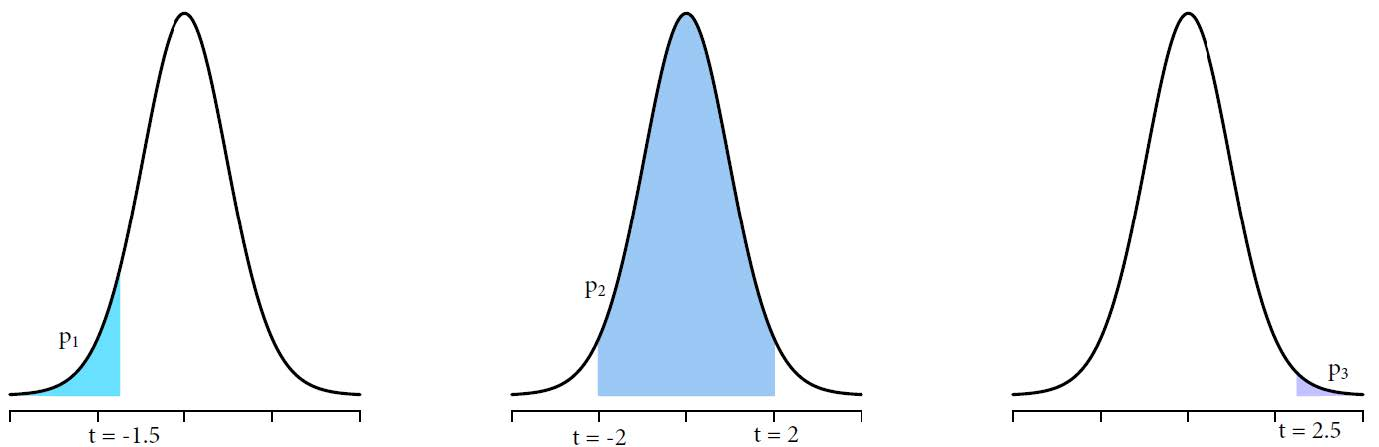
\includegraphics[width=\textwidth]{Files/Images/tdistributions3.jpg}
\end{center}

\clearpage % Page break

\question{
    5.2 g
}{
    For the situation where there are 11 \concept{degrees of freedom}, use the \rcode{pt()} function to get the probabilities p$_1$, p$_2$, and p$_3$ (area under the curve) for the three situations shown in the figures above.
}

\hint{Hint 5.5: For the picture in the middle and the right keep in mind that the \rcode{pt()} function by default uses the left tail and the total area under the curve is 1.}

\rcodeanswermedium{5.2g}

\emptyanswerbox{
    5.2g
}{
    p$_1$: \tinyanswerline \hspace*{2cm} p$_2$: \tinyanswerline \hspace*{2cm} p$_3$: \tinyanswerline
}

When you test a value for a \concept{population mean}, there exist three types of tests: \\

\begin{minipage}[t]{0.33\textwidth}
Two-tailed inequality test: \\
\\
$H_0: \mu = \mu_0$ \\
$H_1: \mu \neq \mu_0$
\end{minipage}
\begin{minipage}[t]{0.33\textwidth}
One-tailed right sided test: \\
\\
$H_0: \mu \leq \mu_0$ \\
$H_1: \mu > \mu_0$
\end{minipage}
\begin{minipage}[t]{0.33\textwidth}
One-tailed left sided test: \\
\\
$H_0: \mu \geq \mu_0$ \\
$H_1: \mu < \mu_0$
\end{minipage}
\vspace*{0.5cm}

\question{
    5.2 h
}{
    Give a critical \concept{t-value} for the three tests described above using a confidence of 98\% and 28 \concept{degrees of freedom}.
}

\hint{Hint 5.6: Use the \rcode{qt()} function in \texttt{R}}.

\rcodeanswermedium{5.2h}

\emptyanswerbox{
    5.2h
}{
    Two-tailed inequality test: \shortanswerline 
    \answerskip
    One-tailed right sided test: \hspace*{-5pt}\shortanswerline 
    \answerskip
    One-tailed left sided test: \shortanswerline 
}

\clearpage % Page break

Three $n = 29$ \concept{samples} were done on three different populations and the \concept{t-score} based on these \concept{samples} was calculated:

\begin{minipage}[t]{0.33\textwidth}
Two-tailed inequality test: \\
\\
$H_0: \mu = 50$ \\
$H_1: \mu \neq \50$ \\
\\
$t = 2.6$
\end{minipage}
\begin{minipage}[t]{0.33\textwidth}
One-tailed right sided test: \\
\\
$H_0: \mu \leq \50$ \\
$H_1: \mu > \50$ \\
\\
$t = -2.3$
\end{minipage}
\begin{minipage}[t]{0.33\textwidth}
One-tailed left sided test: \\
\\
$H_0: \mu \geq \50$ \\
$H_1: \mu < \50$ \\
\\
$t = 1.6$
\end{minipage}
\vspace*{0.5cm}

\question{
    5.2 i
}{
    Using a confidence of 98\%, find out whether the \concept{null hypothesis} $H_0$ is rejected for each of these three cases.
}

\hint{Hint 5.7 : Use the \concept{critical t-values} from the previous assignment and compare these with the sample \concept{t-scores} to draw your conclusion for each of these outcomes.}

\emptyanswerbox{
    5.2i
}{
    Two-tailed inequality test: \hspace*{1.5cm} \textbf{$H_0$ rejected} / \textbf{$H_0$ not rejected}
    \answerbreak
    Explanation: \rule{.75\textwidth}{0.4pt}
    \answerskip
    \answerskip
    One-tailed right sided test: \hspace*{-5pt}\hspace*{1.5cm} \textbf{$H_0$ rejected} / \textbf{$H_0$ not rejected}
    \answerbreak
    Explanation: \rule{.75\textwidth}{0.4pt}
    \answerskip
    \answerskip
    One-tailed left sided test: \hspace*{1.5cm} \textbf{$H_0$ rejected} / \textbf{$H_0$ not rejected}
    \answerbreak
    Explanation: \rule{.75\textwidth}{0.4pt}    
}

\clearpage % Page break
%%%%%%%%%%%%%%%%%%%%%%%%%%%%%%%%%%%%%%%%%%%%%%%%%%%%%%%%%%%%%%%%%%%%%%%%%%%
% Assignment 5.3: Independent two-sample t-test by hand and in R
%%%%%%%%%%%%%%%%%%%%%%%%%%%%%%%%%%%%%%%%%%%%%%%%%%%%%%%%%%%%%%%%%%%%%%%%%%%

\handassignment{Assignment 5.3: Independent two-sample t-test by hand and in R}

To test the effect of caffeine on the respiratory exchange ratio (RER), 9 men get caffeine and 9 different men get a placebo, their RER is measured while doing sports\footnote{These data are taken from \url{http://learntech.uwe.ac.uk/da/Default.aspx?pageid=1438}}: \\
\vspace*{0.5cm}
\begin{center}
\begin{tabular}{c|ccc}
RER measurement & $n$ & Mean ($\bar{x}$) & Standard deviation ($s_x$) \tstrut\bstrut\\
\hline
Caffeine & 9 & 94.22 & 5.61 \tstrut\bstrut\\
Placebo & 9 & 100.56 & 7.70 \tstrut\bstrut\\
\end{tabular}
\end{center}
\vspace*{0.5cm}

Researchers want to use this experiment to show with 95\% confidence that caffeine reduces the RER in men. They are going to evaluate the results by comparing the \concept{mean} RER using a \concept{two-sample t-test}. \\

\question{
    5.3 a
}{
    Why is this test also called an \concept{independent samples t-test}?
}

\twolineanswerbox{5.3a}

\question{
    5.3 a
}{
    Write down the \concept{null hypothesis} $H_0$ and the \concept{alternative hypothesis} $H_1$ for a one-sided test where the researchers want to show that the placebo \concept{mean} RER is higher than the caffeine \concept{mean} RER.
}

\hypothesesbox{5.3b}

In the formula sheet on page~\pageref{formulasheet} you can see that for \concept{independent samples t-tests}:
\vspace*{0.5cm}
\begin{equation*}
    t = \frac{(\bar{x}_1 - \bar{x}_2) - D_0}{\sqrt{s^2_p (\frac{1}{n_1} + \frac{1}{n_2})}}
    \hspace*{3cm}
    s^2_p = \frac{(n_1 - 1) s^2_1 + (n_2 - 1) s^2_2}{n_1 + n_2 - 2}
\end{equation*}
\vspace*{0.5cm}

\question{
    5.3 c
}{
    Using the formula provided calculate the \concept{pooled standard deviation} $s_p$.
}

\clearpage % Page break

\emptyanswerbox{
    5.3c
}{
    $s_p$: \shortanswerline
    \answerskip
    Calculation:
    \answerskip
    \rule{\textwidth}{0.4pt}
}

\question{
    5.3 d
}{
    Using the formula provided calculate the \concept{t-score}.
}

\emptyanswerbox{
    5.3c
}{
    t-score: \shortanswerline
    \answerskip
    Calculation:
    \answerskip
    \rule{\textwidth}{0.4pt}
}

The \concept{critical t-value} for 16 \concept{degrees of freedom} $(n_1 + n_2 - 2)$ for a one-sided test is 1.746. \\

\question{
    5.3 e
}{
    Draw the conclusion for this test. Include the following elements:
        \begin{itemize}
        \item[$\square$] Show how the calculated \concept{t-score} relates to the \concept{critical t-score}.
    \item[$\square$] Discuss whether $H_0$ is rejected or not.
    \item[$\square$] Describe what this tells us about $\mu$ and $\mu_0$.
    \item[$\square$] Describe what type of error is relevant \textit{(type-I or type-II)}.
\end{itemize}
}

\sixlineanswerbox{5.3e}

\clearpage % Page break

\begin{minipage}{0.8\textwidth}
Now you will learn how to do the same independent t-test in \texttt{R}. \\

Run the following code in \texttt{R}: \\
\end{minipage}%
\hfill%
\begin{minipage}{0.1\textwidth}

\includegraphics[width=\linewidth]{Files/Images/displaycode.pdf}
\end{minipage}
\vspace*{.1cm}

\codeblock{{\color{dataset}\# These are the values for the RER test data set}\\
placebo <- c(105, 119, 100, 97, 96, 101, 94, 95, 98)\\
caffeine <- c(96, 99, 94, 89, 96, 93, 88, 105, 88)}

\question{
    5.3 f
}{
    Calculate the \concept{mean} and \concept{standard deviation} for the \rcode{placebo} and \rcode{caffeine} variables, confirm that your results match with the previous assignment.
}

\rcodeanswermedium{5.3f}

\emptyanswerbox{
    5.3f
}{
    \rcode{placebo} \hspace*{6cm} \rcode{caffeine}
    \answerskip
    Mean: \hspace{90pt}\tinyanswerline \hspace*{2cm}Mean: \hspace{80pt}\tinyanswerline
    \answerskip
    Standard deviation: \tinyanswerline \hspace*{1.95cm}Standard deviation: \tinyanswerline
}

Run the following code in \texttt{R}: \\

\codeblock{t.test(x = placebo, y = caffeine, alternative = \textquotesingle greater\textquotesingle, mu = 0, \\
       \hspace*{40pt}paired = FALSE, var.equal = TRUE, conf.level = 0.95)}

\question{
    5.3 g
}{
    Interpret the \texttt{R} code above and check if the results match your conclusion for assignment 5.3e.
}

\twolineanswerbox{5.3g}

The \concept{t-test} assumes equal \concept{variances}. In this case the \concept{standard deviations} are actually a bit different. \\

\clearpage % Page break

\question{
    5.3 h
}{
    Change the \rcode{var.equal} argument in the \texttt{R} code above to do a \concept{Welch t-test} to account for unequal \concept{variances}. Check whether the results differ.
}

\rcodeanswertiny{5.3h}

\twolineanswerbox{5.3h}

\question{
    5.3 i
}{
    How can you check if you need to do a \concept{Welch t-test} instead of a normal \concept{t-test}?
}

\twolineanswerbox{5.3i}

\clearpage % Page break
%%%%%%%%%%%%%%%%%%%%%%%%%%%%%%%%%%%%%%%%%%%%%%%%%%%%%%%%%%%%%%%%%%%%%%%%%%%
% Assignment 5.4: Dependent two-sample t-test in R
%%%%%%%%%%%%%%%%%%%%%%%%%%%%%%%%%%%%%%%%%%%%%%%%%%%%%%%%%%%%%%%%%%%%%%%%%%%

\rassignment{Assignment 5.4: Dependent two-sample t-test in R}

To test for a difference in blood pressure depending on their position, 12 people’s blood pressure was measured twice, first standing up and then lying down. Researchers want to use this experiment to show with 92.5\% confidence that the blood pressure lying down is significantly higher than standing up. They are going to evaluate the results by comparing the \concept{mean} using a \concept{two-sample t-test}. \\

\question{
    5.4 a
}{
    Why is this a dependent (also called paired) \concept{t-test}?
}

\twolineanswerbox{5.4a}

Run the following code in \texttt{R}: \\

\codeblock{{\color{dataset}\# These are the values for the blood pressure data set} \\
standing <- c(132, 146, 135, 141, 139, 162, 128, 137, 145, 151, 131, 
              143) \\
lying <- c(136, 145, 140, 147, 142, 160, 137, 136, 149, 158, 120, 150)}

\question{
    5.4 b
}{
    Calculate the \concept{mean} of the \rcode{standing} and \rcode{lying} data sets, also calculate the differences and the \concept{mean} of the differences.
}

\rcodeanswersmall{5.4b}

\emptyanswerbox{
    5.4b
}{
    Mean standing: \quad \shortanswerline
    \answerskip
    Mean lying: \qquad \quad \shortanswerline
    \answerskip
    Mean difference: \shortanswerline
}

\clearpage % Page break

\question{
    5.4 c
}{
    Write down the \concept{null hypothesis} $H_0$ and \concept{alternative hypothesis} $H_1$ for a one-sided test where the researchers want to show with 92.5\% confidence that the \concept{mean} blood pressure is higher lying down than standing up.
}

\hypothesesbox{5.4c}

Run the following code in \texttt{R}: \\

\codeblock{t.test(x = standing, y = lying, alternative = \textquotesingle greater\textquotesingle, mu = 0 , \\
       \hspace*{40pt}paired = TRUE, conf.level = 0.925)}
       
\question{
    5.4 d
}{
    Check the results of this test. The outcome is a bit strange, can you explain what is wrong here?
}

\onelineanswerbox{5.4d}

\question{
    5.4 e
}{
    Fix the \texttt{R} code to do a correct test and draw the correct (four part) conclusion.
}

\rcodeanswersmall{5.4e}
\sixlineanswerbox{5.4e}

\clearpage % Page break

\vspace*{2cm}
\fancyhf[rh]{}
\begin{center}
    \textit{This page is intentionally left blank}
\end{center}

\clearpage % Page break